\documentclass[11pt]{article}
\usepackage[margin=0.95in]{geometry}
\usepackage[T1]{fontenc}
\usepackage{lmodern}
\usepackage{amsmath,amssymb}
\usepackage{booktabs}
\usepackage{graphicx}
\usepackage[numbers,sort&compress]{natbib}
\setlength{\bibsep}{1pt}
\renewcommand{\bibfont}{\small}
\usepackage[hidelinks]{hyperref}
\usepackage{xcolor}
\usepackage{enumitem}
\setlist{itemsep=2pt,topsep=4pt}
\graphicspath{{../figures/}{figures/}}

\title{Benchmarks Are Measurement Instruments:\\Reliability, Invariance and Validity Ceilings\\for LLM and Agent Evaluation}
\author{Abhay Mettu\\\small\texttt{github.com/abhaymettu/benchmeasure}}
\date{November 2026}

\begin{document}
\maketitle

\begin{abstract}
A benchmark score is a measurement, and psychometrics asks three questions of any measurement: does the score replicate (reliability), does an item mean the same thing for every group measured (invariance), and how much of the thing we care about can the score predict (validity). We put LLM and agent evaluations through all three using only public item-level data, and release a tool that answers them for any models-by-tasks results file.
On SWE-bench Verified (173 public submissions by 500 tasks), reliability is a property of the comparison, not of the benchmark. The share of score variance that reflects real differences between systems (the G coefficient of generalizability theory) is 0.994 across the whole leaderboard and about 0.68 among the leading 20 submissions. Computed the usual way, on the same tasks that picked the leaders, it is 0.19 for the top 10: a winner's curse, which estimating on held-out tasks removes. None of the 19 adjacent pairs in the top 20 differ significantly.
Twelve models run with the same scaffold on SWE-bench Verified and SWE-bench Multilingual let us estimate how much of the second benchmark's signal the first one captures instead of assuming it: the correlation corrected for both scores' noise is 0.98 (0.90 without the weakest model). In this matched set the noise terms outweigh uncovered variance, which suggests that for near transfer, measurement noise, not narrow coverage, limits what the score predicts, the reverse of what our earlier analysis concluded from assumed inputs.
Item-level differential functioning between model families is large on the Open LLM Leaderboard (6 to 10 times sampling noise) and modest on SWE-bench between open- and closed-weight models, and in both it cancels in full scores and returns in subsets: one 50-task subset chosen on other models moves the open versus closed gap by up to 4.7 points against a full-test gap of 1.2.
For the scorer itself, on the MT-Bench comparisons where a like-for-like human ceiling can be computed (one annotator against the majority of the others, 88.2\%), a GPT-4 judge agrees with the human majority 83.4\% of the time in one presentation order and 87.1\% when both orders are averaged, and its order-reversal flip rate (16.1\%) matches its disagreement with itself on identical reruns (16.2\%).
\end{abstract}

\section{Introduction}

Every leaderboard comparison carries three silent assumptions. The first is that the score would come out the same if the evaluation were run again on a fresh sample of similar tasks. The second is that a task means the same thing for every model, so that two models with the same ability have the same chance of solving it whatever family they come from. The third is that the score predicts something outside the benchmark. Psychometrics names these reliability, measurement invariance and validity, and has standard tools for each: generalizability theory for reliability \citep{cronbach1972dependability,brennan2001generalizability}, differential item functioning (DIF) tests for invariance \citep{holland1988dif,swaminathan1990logistic,meredith1993measurement}, and the attenuation bound for validity \citep{spearman1904proof}.

This paper treats an evaluation as an instrument with three parts: a set of tasks, a scorer that turns a model's output into a grade, and repeated runs. Each part can fail as a measurement, and we measure each failure on public data. It unifies three open repositories into one programme and one tool:
\begin{itemize}
\item \textbf{Reliability and the validity ceiling} on SWE-bench \citep{jimenez2024swebench} Verified, a human-curated subset of 500 tasks \citep{yang2025swesmith},, with variance components estimated from 173 public submissions and coverage estimated from SWE-bench Multilingual \citep{yang2025swesmith} (repository \texttt{agent-validity-ceiling}, extended here).
\item \textbf{Invariance}: classical DIF on 395 Open LLM Leaderboard models from the tinyBenchmarks release \citep{polo2024tinybenchmarks}, and the same checks on SWE-bench (repository \texttt{benchdif}).
\item \textbf{The scorer}: an LLM judge calibrated against the human-to-human ceiling on MT-Bench \citep{zheng2023judging} (repository \texttt{judge-reliability}).
\end{itemize}

\paragraph{Contributions.} (1) A reliability curve for SWE-bench Verified across comparison populations, and the observation that estimating a leading group's reliability on the scores that selected it is strongly biased low, with a split-task estimator and a cross-check. (2) A validity ceiling $R^2 \le \rho_X \rho_Y C$ whose inputs, including coverage $C$, are estimated from matched item-level data rather than assumed, used to attribute the gap between benchmark and criterion to its sources. (3) Evidence on two very different benchmarks that item-level DIF cancels in full scores but not in subsets, including the published 50-task SWE-bench Verified Mini. (4) \texttt{benchmeasure}, a command-line tool that reports all three properties for any models-by-tasks results file in one command.

\paragraph{What is not new.} Generalizability theory has been applied to agent benchmarks \citep{srinivasan2026ddr,hardy2026agentreliability}, including a 50-task SWE-bench Verified subset with a scaffold facet \citep{hardy2026agentreliability}. Liu et al.\ \citep{liu2026converged} audited 254 public SWE-bench submissions and found that exact McNemar tests separate none of the 29 adjacent top-30 Verified pairs; we reproduce that count on our matrix. Zheng and Yang \citep{zheng2026familydif} report the same qualitative DIF pattern (robust aggregate rankings, fragile near-ties) with a multidimensional IRT approximation. Judge-versus-human agreement is well studied \citep{zheng2023judging,thakur2025judging,bavaresco2024judgebench}, and G-theory for LLM-judged benchmarks has been done at scale \citep{anand2026askwhich}. Multiplicative validity bounds have been argued from surveys \citep{caban2026measurement}, and Li and Ni \citep{li2026measuredorreal} show the Spearman correction can be unstable, which is why we report the coverage estimate with its interval and its sensitivity to single models. Our contribution is the combination: one measurement model across tasks, runs and scorers, every input estimated from public item data, and the winner's-curse correction.

\section{A measurement model for evaluation scores}
\label{sec:model}

Let $x_{mi}$ be the score of model (or model and scaffold system) $m$ on task $i$, $0/1$ for pass or fail. With every model attempting every task once, the two-way random effects model is
\begin{equation}
x_{mi} = \mu + \alpha_m + \beta_i + (\alpha\beta)_{mi,e},
\end{equation}
with variance components $\sigma^2_m$ (true differences between models), $\sigma^2_i$ (task difficulty) and $\sigma^2_{mi,e}$ (model by task interaction confounded with run noise). They are estimated from the ANOVA mean squares. The leaderboard score is the row mean $\bar x_m$, and its reliability for ranking models, the G coefficient, is
\begin{equation}
E\rho^2 = \frac{\sigma^2_m}{\sigma^2_m + \sigma^2_{mi,e}/n_i},
\label{eq:g}
\end{equation}
which equals Cronbach's alpha computed over tasks. The standard error of measurement of a score is $\sqrt{\sigma^2_{mi,e}/n_i}$. Two facts make Eq.~\ref{eq:g} useful for evaluation. It depends on $\sigma^2_m$, the spread of the models being compared, so the same 500 tasks can be very reliable for one comparison and unreliable for another. And it projects: replacing $n_i$ gives the reliability with more or fewer tasks (a decision study).

When repeated runs exist, a third facet $r$ separates run noise from stable interaction ($\sigma^2_{mi}$, $\sigma^2_{mr}$, $\sigma^2_{mir,e}$), and the error term becomes $\sigma^2_{mi}/n_i + \sigma^2_{mr}/n_r + \sigma^2_{mir,e}/(n_i n_r)$. A judged benchmark adds a rater facet in the same way. Public SWE-bench submissions have one run each, so we bound the run share with external estimates \citep{bjarnason2026randomness}.

\paragraph{Invariance.} DIF is structure in the interaction term that follows a grouping of models: task $i$ is easier for group $A$ than group $B$ at equal ability. We use logistic regression DIF matched on total score \citep{swaminathan1990logistic} with Benjamini-Hochberg control, and two test-level summaries. The \emph{excess gap variance} compares the variance across tasks of the per-task group gap $\bar x_{Ai} - \bar x_{Bi}$ with its expectation under binomial noise alone; a ratio of 1 means no DIF, and $1 - 1/\text{ratio}$ is the task-specific share. Because a difference in ability alone makes per-task gaps uneven on the probability scale, we also compute the ratio within bands of total score. The \emph{held-out subset shift} picks, on half of each group's models, the $k$ tasks that most favour each group, and measures on the other half how far each subset moves the group gap from its full-test value; the \emph{swing} is the difference between the two subsets' gaps. Selection and measurement use different models, split by base model where one model appears under several scaffolds.

\paragraph{Validity ceiling.} If $\rho_X$ and $\rho_Y$ are the reliabilities of a benchmark score and a criterion, and $C$ is the squared correlation of their true scores (the share of the criterion's true variance that the benchmark's construct covers), then attenuation gives
\begin{equation}
R^2_{XY} \le \rho_X\, \rho_Y\, C,
\label{eq:ceiling}
\end{equation}
and the unit total of the criterion's variance splits into benchmark noise $1-\rho_X$, criterion noise $\rho_X(1-\rho_Y)$, uncovered variance $\rho_X\rho_Y(1-C)$ and the reachable ceiling. Our earlier analysis, in the agent-validity-ceiling repository, applied Eq.~\ref{eq:ceiling} with run-to-run variance from the literature, between-model variance read off the leaderboard by eye, and assumed coverage values of 0.15 to 0.40. Here $\rho_X$ and $\rho_Y$ come from Eq.~\ref{eq:g} and $C$ from the disattenuated correlation between two benchmarks run on the same models.

\section{Data}

\textbf{SWE-bench Verified and Multilingual.} We built item response matrices from the public \texttt{SWE-bench/experiments} repository (commit \texttt{40f164d}, September 2026), which holds a per-task resolved list for each leaderboard submission. Verified gives 173 submissions by 500 tasks, dated October 2023 to September 2026, with resolve rates from 0.4\% to 79.2\%. We dropped two submissions whose per-task files contradict their reported score (10.2\% against a reported 52.8\%, and 0.0\% against 69.6\%). Multilingual gives 14 submissions by 300 tasks. Twelve models were run on both with the same scaffold release (mini-SWE-agent v2), which is the matched set for coverage. A submission is a model and scaffold system; many models appear under several scaffolds.

\textbf{Open LLM Leaderboard.} Per-item correctness for 395 models from the tinyBenchmarks release \citep{polo2024tinybenchmarks}, used in \texttt{benchdif}. Families are parsed from model names: Llama-2 derived ($n=38$) against Mistral derived ($n=41$).

\textbf{MT-Bench human judgments.} 1814 pairwise comparisons with 3355 votes from 65 annotators over 80 questions and 6 models, with the GPT-4 judgments released alongside \citep{zheng2023judging}, used in \texttt{judge-reliability}.

\section{Reliability depends on the comparison}

\subsection{The reliability curve and a winner's curse}

Table~\ref{tab:curve} and Figure~\ref{fig:curve} give the G coefficient of the SWE-bench Verified ranking as the compared set narrows from all 173 submissions to the leading 10. Across the whole board the true spread between submissions is 19.1 points against a score standard error of 1.5, and $E\rho^2 = 0.994$. The rank order of the leaderboard as a whole is real. Among the top 50 (scores 68\% to 79\%) the spread falls to 2.8 points and $E\rho^2 = 0.85$; among the top 20 it is 1.6 points and $E\rho^2 = 0.68$.

The obvious way to compute the top-$k$ figure, picking the leading $k$ and running Eq.~\ref{eq:g} on their 500 scores, gives much lower numbers: 0.50 for the top 20 and 0.19 for the top 10. Those are biased low. A model makes the top 10 partly because its noise ran high, so within the selected set noise and true score are negatively related, the observed spread is compressed, and $\sigma^2_m$ is understated. This is the reliability version of the winner's curse. Separating selection from measurement removes it: pick the top $k$ on a random half of the tasks, estimate the variance components on the other half, and project to 500 tasks with Eq.~\ref{eq:g}. The split estimate has a smaller bias in the other direction, because selecting on 250 tasks is noisier than selecting on 500, so the chosen set reaches a little further down the board and is more spread out than the true top $k$. A cross-check that uses no variance components agrees: the correlation of the chosen models' scores on the two halves, stepped up to 500 tasks with the Spearman-Brown formula, is 0.69 for the top 20 and 0.61 for the top 10. We therefore read the top-20 reliability as about 0.68 and the top-10 reliability as somewhere between 0.6 and 0.7, and the naive figures as a warning about how reliability is usually computed for leaders.

\begin{table}[t]
\centering
\small
\begin{tabular}{lrrrrrrr}
\toprule
compared set & scores & model SD & SEM & split & halves & naive & tasks for 0.9 \\
\midrule
all 173 & 0.4 to 79.2 & 19.10 & 1.50 & 0.994 & 0.995 & 0.994 & 28 \\
top 100 & 53.2 to 79.2 & 7.52 & 1.34 & 0.969 & 0.972 & 0.968 & 143 \\
top 50 & 68.2 to 79.2 & 2.83 & 1.18 & 0.852 & 0.845 & 0.830 & 781 \\
top 30 & 71.8 to 79.2 & 2.35 & 1.15 & 0.808 & 0.762 & 0.701 & 1067 \\
top 20 & 74.4 to 79.2 & 1.63 & 1.11 & 0.682 & 0.686 & 0.502 & 2096 \\
top 10 & 75.8 to 79.2 & 1.63 & 1.09 & 0.690 & 0.610 & 0.194 & 2023 \\
\bottomrule
\end{tabular}
\caption{Reliability of the SWE-bench Verified ranking by compared set. Scores, SD and SEM in percentage points. Split: top $k$ chosen on half the tasks, variance components estimated on the other half (medians over 50 splits), projected to 500 tasks. Halves: correlation of the chosen models' half-test scores, stepped up to 500 tasks. Naive: chosen and estimated on the same tasks. Tasks for 0.9: tasks needed for $E\rho^2 = 0.9$ at the split estimate's spread (a decision study).}
\label{tab:curve}
\end{table}

\begin{figure}[t]
\centering
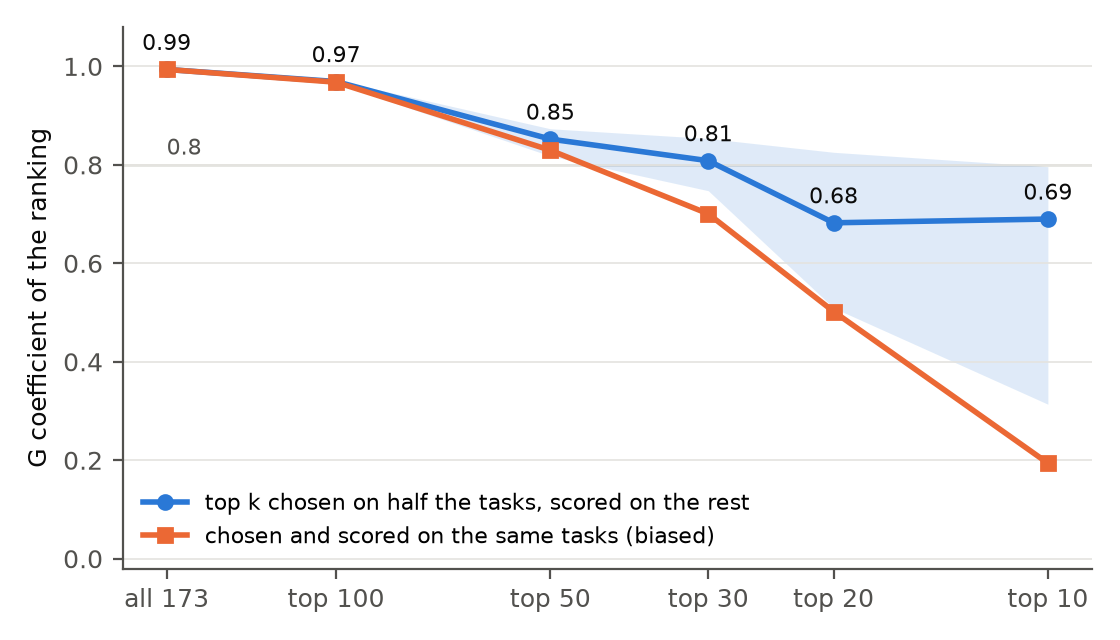
\includegraphics[width=0.7\linewidth]{fig_reliability_curve.png}
\caption{G coefficient of the SWE-bench Verified ranking as the compared set narrows. The band is the 10th to 90th percentile over 50 task splits. Choosing and scoring the leaders on the same tasks (orange) understates reliability.}
\label{fig:curve}
\end{figure}

Frontier sets defined without looking at scores avoid selection altogether. The eleven models in the February 2026 mini-SWE-agent v2 batch, one scaffold and scores from 56\% to 77\%, have $E\rho^2 = 0.96$ (bootstrap interval 0.74 to 0.98), as do the twelve submissions from 2026 (0.95). The benchmark separates frontier models that differ by several points well. What it cannot do is order a cluster of systems within two or three points of each other, which is exactly the comparison a new state-of-the-art claim makes.

\subsection{Pairs}

The same conclusion holds for individual comparisons. With exact McNemar tests on the shared tasks \citep{mcnemar1947note}, none of the 19 adjacent pairs in the top 20 is separable at $\alpha = 0.05$, and none of the 29 in the top 30, which matches the count of Liu et al.\ \citep{liu2026converged}. Across all 190 top-20 pairs, 15.3\% are separable before any correction for multiple tests, against 5\% expected by chance alone. The median adjacent gap is 0.2 points with 59 discordant tasks; at that discordance the smallest true gap a paired test detects with 80\% power is 4.3 points, about the whole top-20 spread of 4.8.

\subsection{Runs or tasks}

With one run per submission, run noise lands in two places. Run-to-run variation in a system's overall level ($\sigma^2_{mr}$) is absorbed into $\sigma^2_m$, which makes the G coefficients above somewhat optimistic about what a rerun would show; run-to-run variation on individual tasks ($\sigma^2_{mir}$) sits in the residual. Bjarnason et al.\ \citep{bjarnason2026randomness} ran 10 full repetitions of SWE-bench Verified for 12 model, scaffold and temperature configurations and found run-to-run standard deviations of the score of 0.7 to 1.8 points. The top-20 single-run SEM here is 1.11 points. If the run-to-run SD of current leaders were at the low end, 0.7 points, and all of it task-level, run noise would be 40\% of the residual and averaging five runs would raise top-20 reliability from 0.68 to 0.76. The published SDs above 1.1 points cannot all be task-level noise for these systems, since they would exceed the whole residual; those configurations are weaker models than today's leaders, so the frontier value is unknown. Either way, a claim of a one or two point improvement at the top of SWE-bench Verified needs repeated runs and a paired test, and the decision study in Table~\ref{tab:curve} says that adding tasks alone would take about 2000 of them to reach 0.9.

\section{Invariance: differential functioning cancels in full scores and returns in subsets}

\subsection{Open LLM Leaderboard}

On the 79 Llama-2 and Mistral derived models, logistic regression DIF flags 154 to 777 items per benchmark at a false discovery rate of 0.05, and 571 of 1534 on MMLU professional law. The effect is not multiplicity or model dependence: permuting family labels at the level of lineages (single-linkage clusters of near-duplicate fine-tunes) flags a median of 2 professional-law items against 571, and the per-item family gap has 6.1 to 9.7 times the variance that binomial noise predicts across five benchmarks, so 84 to 90\% of the per-item family difference is item specific.

It cancels at the test level. Of the 571 flagged professional-law items, 278 favour Mistral and 293 favour Llama-2; dropping all of them moves the family accuracy gap from 0.0216 to 0.0221 and the mean model rank by 3.6 places of 79. Subsets do not inherit this protection. Choosing on half the models the 100 items that most favour each family and scoring both subsets on the other half, the two subsets' family gaps differ by 0.51 to 0.95 across the five benchmarks, against full-benchmark gaps of 0.0005 to 0.19, and random 100-item subsets reverse the sign of the family ordering in 65 of 400 draws on professional law. Individual flags are noisy (about 40\% replicate on held-out models against a base rate of 13 to 22\%), so the claim is about the aggregate, not any single item. Mantel-Haenszel is inapplicable on these matrices: with 79 models and about 1500 score levels the strata are nearly empty, the transpose of the usual psychometric shape.

\subsection{SWE-bench Verified}

Between the 35 open-weight and 138 closed-weight submissions the pattern repeats with a smaller effect. The per-task gap has 1.29 times its sampling variance; computed within five bands of total score, which removes the inflation that a difference in ability alone produces on the probability scale, it is 1.39 times (28\% task specific). Logistic DIF flags 8 of 500 tasks. The full-score gap is $-1.2$ points. Splitting submissions by base model (129 distinct), so that one model under two scaffolds never sits on both sides, a 50-task subset chosen on one half moves the gap on the other half by up to 4.7 points on average, about four times its size, and the two most adversarial 50-task subsets differ by 8.2 points. Random 50-task subsets reverse the gap's sign in 12.5\% of draws.

The published SWE-bench Verified Mini (50 tasks) preserves the open versus closed gap ($-1.2$ points on both) and the overall ranking (Spearman 0.95 over all 173 submissions). Its ranking of the top 20 correlates 0.36 with the full benchmark's, which is typical of any 50 tasks: random 50-task subsets give a median of 0.42 (10th to 90th percentile 0.09 to 0.67), and the projected top-20 reliability at 50 tasks is 0.18. Mini is as good a 50-task sample as any; no 50-task sample can rank leaders.

\paragraph{Repository mix.} Splitting the tasks into Django (231) and the rest (269), the two halves' true-score correlation is 0.99 across all submissions but 0.77 across the top 50, with a bootstrap interval of 0.47 to 1.02 that includes 1. We read this as a possible model by repository interaction among leaders that this sample cannot confirm.

\section{The scorer: an LLM judge is a rater with its own reliability}

When the scorer is an LLM judge, the judge is a facet of the measurement, and its reliability bounds everything downstream. The right comparison is the reliability of the human labels it replaces, on the same items. On the MT-Bench human judgments with ties excluded, the usual human baseline, one annotator against another, is 82.7\%. But a judge is scored against a majority, a denoised label, so the like-for-like ceiling is one annotator against the majority of the others: 88.2\% (95\% interval 84.9 to 91.0), computed on the 249 comparisons that have enough annotators. On exactly those comparisons, GPT-4 judging a pair in one presentation order agrees with the human majority 83.4\% of the time, 4.8 points below the ceiling (paired interval $-9.6$ to $+0.1$). Judging both orders and averaging brings it to 87.1\%, 1.1 points below (interval $-5.7$ to $+3.5$). Single-answer grading reaches 93.4\%, above the ceiling, but only on the 151 comparisons where it does not call a tie, which are easier. Over all 1192 comparisons where it decides, one-order agreement is 85.5\%, against 70.6\% for a rule that always picks the longer answer. Cohen's kappa \citep{cohen1960kappa} is 0.47 for GPT-4, 0.24 for the length rule and 0.02 for a coin; Krippendorff's alpha \citep{krippendorff2004reliability} over the 65 annotators is 0.485, and adding GPT-4 to the pool moves it to 0.477. On this evidence a swap-averaged GPT-4 judge is about as reliable as one more careful human annotator, and a single-order judge is somewhat less.

Its biases look different next to its own noise. Reversing the presentation order flips the verdict on 16.1\% of 1814 comparisons, and GPT-4 picks the first-shown answer 50.7\% of the time, so there is no net preference for either position. On the 1356 judgments that exist twice in the released files with identical prompts, GPT-4 disagrees with itself 16.2\% of the time. Order flips are therefore no more frequent than the judge's run-to-run disagreement, which is why swap averaging, which recovers 2.9 points of agreement, behaves like variance reduction (the run facet of Section~\ref{sec:model}). This does not rule out position effects at the level of single items that cancel in aggregate; it shows that their net size cannot be told apart from rerun noise here. Verbosity is similar: GPT-4 picks the longer answer 70.5\% of the time and so do the humans (70.6\%), so the judge's correlation with length is not by itself evidence of bias. Self-preference survives the comparison with humans in part: GPT-4 rates its own family's answers 12.7 points above the human win rate (9.5 to 16.0, 578 comparisons) against 3.9 points for a Claude control. The judge also separates other models more sharply than the humans do, and the control family is weaker, so part of the 12.7 points may be decisiveness rather than self-preference.

\section{Validity ceilings with measured inputs}

\begin{figure}[t]
\centering
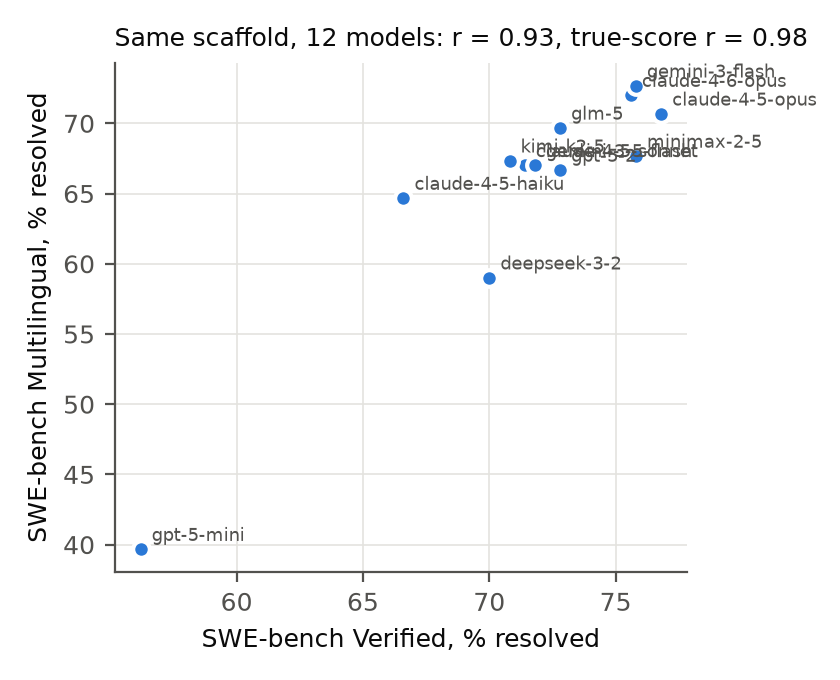
\includegraphics[width=0.48\linewidth]{fig_multilingual.png}
\caption{Twelve models run with the same scaffold release on SWE-bench Verified (500 Python tasks) and SWE-bench Multilingual (300 tasks in other languages).}
\label{fig:ml}
\end{figure}

The twelve matched models (Figure~\ref{fig:ml}) score 56\% to 77\% on Verified and 40\% to 73\% on Multilingual. The observed correlation is 0.93. The G coefficients within this set are 0.953 for Verified and 0.954 for Multilingual, so the true-score correlation is 0.978 and coverage $C = 0.96$, with a model-bootstrap interval of 0.63 to 1.00.

One property of Eq.~\ref{eq:ceiling} needs stating plainly. When $\rho_X$, $\rho_Y$ and $C$ are all estimated on the same models, the ceiling equals the observed $R^2$ by construction ($0.953 \times 0.954 \times 0.956 = 0.869 = 0.932^2$): within a population the bound is attained. The ceiling's value is not a new prediction but an attribution of the shortfall from 1 to its three sources, and a transfer of $C$ to settings where only reliabilities are known.

\begin{table}[t]
\centering
\small
\begin{tabular}{lrrrrrrr}
\toprule
matched set & $\rho_X$ & $\rho_Y$ & $C$ (95\% CI) & $X$ noise & $Y$ noise & uncovered & ceiling \\
\midrule
all 12 & 0.953 & 0.954 & 0.96 (0.63 to 1.00) & 0.047 & 0.044 & 0.040 & 0.869 \\
11, no GPT-5 mini & 0.856 & 0.761 & 0.80 (0.53 to 1.00) & 0.144 & 0.205 & 0.128 & 0.523 \\
\bottomrule
\end{tabular}
\caption{The unit total for predicting SWE-bench Multilingual from SWE-bench Verified in the matched set, split into benchmark noise $1-\rho_X$, criterion noise $\rho_X(1-\rho_Y)$, uncovered variance $\rho_X\rho_Y(1-C)$ and the reachable ceiling $\rho_X\rho_Y C$. Dropping the weakest model narrows the spread, which lowers both reliabilities and the coverage estimate.}
\label{tab:ceiling}
\end{table}

Table~\ref{tab:ceiling} gives the attribution. The coverage estimate leans on the weakest model: without GPT-5 mini the spread narrows, both reliabilities fall, and $C$ drops to 0.80 (0.53 to 1.00). In both rows the two noise terms together (0.09 and 0.35) are larger than the uncovered term (0.04 and 0.13). For near transfer, then, the evidence suggests that what limits the predictive power of SWE-bench Verified scores is measurement noise rather than what the benchmark leaves out. That is the opposite of the conclusion our earlier analysis reached from assumed inputs (the agent-validity-ceiling repository, which used a central coverage of 0.25 within an assumed range of 0.15 to 0.40, and a frontier reliability of 0.94 from a leaderboard spread estimated by eye). Section 4 shows the frontier spread is about 1.6 points, not 5, so frontier reliability is near 0.7; a criterion measured on the same narrow set would be less reliable still, and so would the ceiling.

Three cautions. Multilingual is near transfer: the same task format, harness and kind of repository-level bug fix, in other languages. Coverage of deployment usefulness is surely lower, and no public data measures it. The disattenuated correlation is unstable when reliabilities are estimated with error \citep{li2026measuredorreal}; we report its bootstrap interval, which reaches the boundary at 1 in both rows, and do not apply the confidence-bound correction Li and Ni propose. And the estimate rests on twelve models from one scaffold release.

\section{Related work}

\textbf{Noise and error bars.} Miller \citep{miller2024errorbars} gives standard errors, paired differences and power for evals treated as samples from a question population; Madaan et al.\ \citep{madaan2024variance} quantify seed variance; Heineman et al.\ \citep{heineman2025signal} define a signal-to-noise ratio close in spirit to a G coefficient. Bjarnason et al.\ \citep{bjarnason2026randomness} measure run-to-run variance on SWE-bench Verified directly.

\textbf{G-theory for agents and judges.} Srinivasan \citep{srinivasan2026ddr} decomposes variance on TheAgentCompany, tau2-bench and AppWorld and finds the agent main effect under 3\% of total variance; Hardy et al.\ \citep{hardy2026agentreliability} decompose 22 agent benchmarks including SWE-bench Verified Mini and show that more tasks cannot fix a ranking whose error is dominated by scaffold coverage. Anand \citep{anand2026askwhich} applies G-theory to 373,019 judge scores and shows a single judge caps generalizability. Our reliability curve, the winner's-curse correction and the link to a validity ceiling are, as far as our searches found, not in these papers.

\textbf{IRT and invariance.} IRT for leaderboards \citep{lalor2016irt,rodriguez2021evaluation,vania2021comparing} and for efficient subsets \citep{polo2024tinybenchmarks,hofmann2025fluid} assumes item parameters shared across models, which DIF tests; Jiang et al.\ \citep{jiang2026trustirt} show IRT estimators built for human testing can misbehave in the few-models, many-items regime. Zheng and Yang \citep{zheng2026familydif} find family DIF with a spectral MIRT approximation. Rater-facet Rasch models have been applied to LLM raters \citep{sachdeva2026rasch}.

\textbf{Validity.} Bean et al.\ \citep{bean2025measuring} review construct validity across 445 benchmarks; Patel et al.\ \citep{patel2026beyond} argue for ranking agents by predictive validity; Caban \citep{caban2026measurement} proposes a multiplicative bound from a survey of agentic evaluations; Cao et al.\ \citep{cao2025codebench} give a rigor checklist for code benchmarks.

\textbf{Judges.} MT-Bench and Chatbot Arena \citep{zheng2023judging,chiang2024arena}, position bias \citep{wang2023notfair}, self-preference \citep{panickssery2024selfpref,wataoka2024selfpref}, judges against humans \citep{thakur2025judging,bavaresco2024judgebench}, replication instability \citep{kumar2026verdicts} and disagreement among MT-Bench's own human pools \citep{jha2026whosegold}.

\section{What to report}

The three checks are cheap once item-level results exist, and each changes a conclusion in the data above. We suggest that a leaderboard or a paper claiming an improvement report:
\begin{enumerate}
\item \textbf{The G coefficient for the comparison being made}, estimated with selection and measurement on different tasks, plus the paired test and the minimum detectable difference for the specific pair.
\item \textbf{Repeated runs} when the claimed gap is within a few SEMs, so that run noise can be separated from task sampling.
\item \textbf{The excess gap variance and held-out subset swing} for any grouping that matters (model family, open versus closed weights, language), and the same for any subset used in place of the full benchmark.
\item \textbf{The scorer's agreement against the like-for-like human ceiling on the same items}, and its own replication agreement, before reading anything into its biases.
\item \textbf{A measured coverage} wherever a second benchmark exists for the same models, with its interval, and the ceiling as a bound.
\end{enumerate}
For any models-by-tasks file, in wide or long format and with optional groups and criterion files, the command
\begin{center}\texttt{benchmeasure report results.csv}\end{center}
prints items 1, 3 and 5, and \texttt{benchmeasure demo} runs it on the SWE-bench matrices used here. Item-level DIF calls \texttt{benchdif}, whose closed-form tests match statsmodels to machine precision.

\section{Limitations}

\begin{itemize}
\item \textbf{Submissions are not a random sample} of systems, and many share a model. The G coefficient describes this leaderboard's population, which is the population its readers compare.
\item \textbf{One run per submission} folds run-level variation into the model variance, which makes the G coefficients somewhat optimistic about reruns, and mixes task-level run noise into the residual; published run variance from different, weaker configurations only bounds the split.
\item \textbf{The split-task reliability estimate is slightly optimistic} for small $k$ (selection on half the tasks is noisier), which the halves cross-check shows at $k = 10$.
\item \textbf{Coverage rests on twelve matched models}, moves from 0.96 to 0.80 when the weakest is dropped, and measures near transfer only. It says nothing about deployment, where no public criterion data exists.
\item \textbf{DIF is a symptom, not a cause.} It can come from training data, tokenization, prompt format or scaffold; nothing here attributes it, and nothing here shows contamination.
\item \textbf{The Open LLM Leaderboard results are 2023 to 2024 models}; the judge results are one judge (GPT-4, June 2023) on one dataset.
\item \textbf{Upstream data quality.} Two SWE-bench submissions had per-task files that contradict their reported scores and were dropped; others may have errors we cannot detect.
\end{itemize}

\section*{Reproducibility}

{\sloppy Every number in Sections 4, 5.2 and 7 is written by \texttt{experiments/swebench.py} to \texttt{results/swebench.json} with fixed seeds, and a test regenerates the file byte for byte. The matrices are rebuilt from the public repository by \texttt{data/build\_swebench.py}. Section 5.1 numbers come from \texttt{benchdif/validation/} scripts and Section 6 from \texttt{judge-reliability}'s \texttt{make analysis}, which regenerates its README from \texttt{output/metrics.json}. All data are public; no model was called for this paper.\par}

\bibliographystyle{plainnat}
\bibliography{refs}

\end{document}
